\documentclass[../main.tex]{subfiles}
\begin{document} \label{chapter_formants}
\par In this chapter, we give an in-depth review of formant trajectory extraction. As seen in section \ref{birdsong_review}, birdsong can be compared to human vowels in structure. Moreover, in subsection \ref{subsection_fmnts} we learned that formants can be useful to characterise human vowels. By establishing this link, it becomes reasonable to argue that formant trajectories would be suitable as feature vectors. 
\par Therefore, we dedicate this chapter to the study of formants, and we do so two-fold: in section \ref{section_dsp}, we present all the tools from Signal Processing required to introduce the concept of formants, and more generally, the Linear Predictive Coding framework, which is introduced in section \ref{section_lpc}. This enables us to give a thorough description of what formants mean, and how to compute them.

\section{Signal analysis review} \label{section_dsp}
In this section, we give an overview of key concepts from Digital Signal Processing (DSP) that will be useful to give a deeper presentation of formants in section \ref{section_lpc}. We first introduce LTI systems and their representation in both, the time and frequency domains. Then, we present autoregressive models, the autocorrelation function, the Yule-Walker equations, which are useful to set out the parameters of an autoreggresive model in terms of the autocorrelation. Next, we present the Levinson-Durbin recursion, which is a technique used to solve these last equations. Finally, we introduce signal preprocessing techniques, which will contribute to the system architecture presented in section \ref{section_form_estimation}. 

\subsection{LTI systems in the time and frequency domains} \label{subsection_lti} 
A discrete-time system's (DTS) definition is very closely linked to that of a discrete function. Any such system contains two sequences, an input sequence $\V{x} = (x_1, x_2, ..., x_n)$ and an output sequence $\V{y} = (y_1, y_2, ..., y_n)$, which are related by a transformation $T$, i.e. $\V{y} = T\{\V{x}\}$.  \cite{Oppenheim2010}. 
\par Some DTS satisfy the properties of linearity and time-invariance, which are given below:
\begin{definition}{Linearity.} \label{def_linearity}
Let $T$ be the transformation of a DTS. We say that this DTS is linear if and only if $T$ is linear, i.e. for all inputs $\V{x, x}'$ and corresponding outputs $\V{y, y}'$, and for all constants $a$, the following hold:
\begin{align*}
T\{\V{x} + \V{x}'\} &= T\{\V{x}\} + T\{\V{x}'\} \\
&= \V{y} + \V{y}'\\
T\{a\V{x}\} &= aT\{\V{x}\}\\
&= a\V{y}
\end{align*}
\end{definition}
\begin{definition}{Time-invariance.} \label{def_ti}
Let $\V{y}$ be the output of a DTSS for input $\V{x}$. This DTS is said to be time-invariant if for all constants $n_0$ the following holds:
\begin{align*}
\forall n_0, x_k = x_{k+n_0} \implies y_k = y_{k+n_0}
\end{align*}
\end{definition}
\par Now, let $\V{\delta}$ be the unit sample sequence, i.e. $\V{\delta}_n = 1 \iff n = 0$, and $\V{\delta}_n = 0$ otherwise. It is easy to see that any element $x_n$ of a sequence $\V{x}$ can be expressed as an infinite sum with the following shape:
\begin{align*}
x_n = \sum_{k=-\infty}^{\infty}x_k\delta_{n-k}
\end{align*}
\par This decomposition is useful to define an LTI system:
\begin{definition}{LTI system.} \label{def_lti}
A DTS is said to be a Linear Time-Invariant (LTI) system if it satisfies the properties of linearity and time-invariance, as given in definitions \ref{def_linearity} and \ref{def_ti}. In other words, for two elements $x_n, y_n$ in sequences $\V{x, y}$, the following is true:
\begin{align*}
y_n &= T\{\sum_{k=-\infty}^{\infty}x_k\delta_{n-k}\}\\
&= \sum_{k=-\infty}^{\infty}x_kT\{\delta_{n-k}\}\\
&= \sum_{k=-\infty}^{\infty}x_kh_{n-k}
\end{align*}
\end{definition} 
\par Where $h_{n}$ is called the impulse response of the system. From this definition, we can conclude that any LTI system is completely characterised by its impulse response \cite{Oppenheim2010}.  
\begin{definition}{Convolution.} \label{def_convolution}
The convolution of two signals $\V{x, h}$ is defined as:
\begin{align*}
\V{y} &= \V{x} \Conv \V{h}\\
\implies y_n &= \sum_{k=-\infty}^{\infty}x_kh_{n-k}, \forall n
\end{align*}
\end{definition}
\par Time signals are often analysed in the frequency domain because this unveils the contribution of different frequency components, which can be useful to distinguish useful information about the signal. In subsection \ref{subsection_fft}, we defined the the Fourier Transform $X = \mathcal{F}\{\V{x}\}$ for discrete signals. We recall that the Fourier Transform is a useful tool to compute the frequency-domain representation of a time signal. We now present some important results about it.
\begin{theorem}{The Convolution Theorem.} \label{theo_conv}
Let $\V{x, h, y}$ be time-domain signals with $y_n = \V{x}\Conv\V{h}, \forall n$. Then, their respective Fourier Transforms $X, H, Y$ satisfy:
\begin{align*}
Y(e^{j\omega}) = X(e^{j\omega})H(e^{j\omega})
\end{align*}
\end{theorem}
\par In the last equation, $H(e^{j\omega})$ is called the frequency response of the LTI system
\begin{theorem}{Parseval's Theorem.} \label{theo_parseval}
Let $X = \mathcal{F}\{\V{x}\}$, where $\V{x}$ is a time-domain signal. Then, the energy density spectrum of $\V{x}$, defined as:
\begin{align*}
E &= \sum_{k=-\infty}^{\infty}\abs{x_n}^2\\
&= \frac{1}{2\pi}\int_{-\pi}^\pi{\abs{X(e^{j\omega})}^2d\omega}
\end{align*}
\end{theorem}
\par One useful way of representing signals is by plotting how much power is contained at each given frequency. This is called a \emph{frequency spectrum}. However, this representation is often used to generate yet another representation, called the \emph{spectral envelope} of the signal, which is a smoothed version of the frequency spectrum. Figure \ref{fig_specenv} shows how these two representations are related.
\begin{figure}[t]
\centering
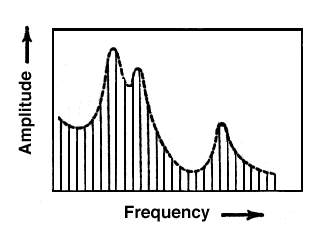
\includegraphics[width=80mm]{specenv}
\caption{The frequency spectrum and its smoothed representation, the spectral envelope (bold line).}
\label{fig_specenv}
\end{figure}
\par Additionally, it is often convenient to analyse how the frequency content changes over time, particularly so when analysing phenomena such as birdsong or human speech, in which signals can only be represented as LTI systems at a specific point in time. The \emph{spectrogram} of a signal is a representation displaying the energy distribution over frequency bins at each point in time that is useful in this scenario. An example of this can be seen in figure \ref{fig_spec}.
\begin{figure}[t]
\centering
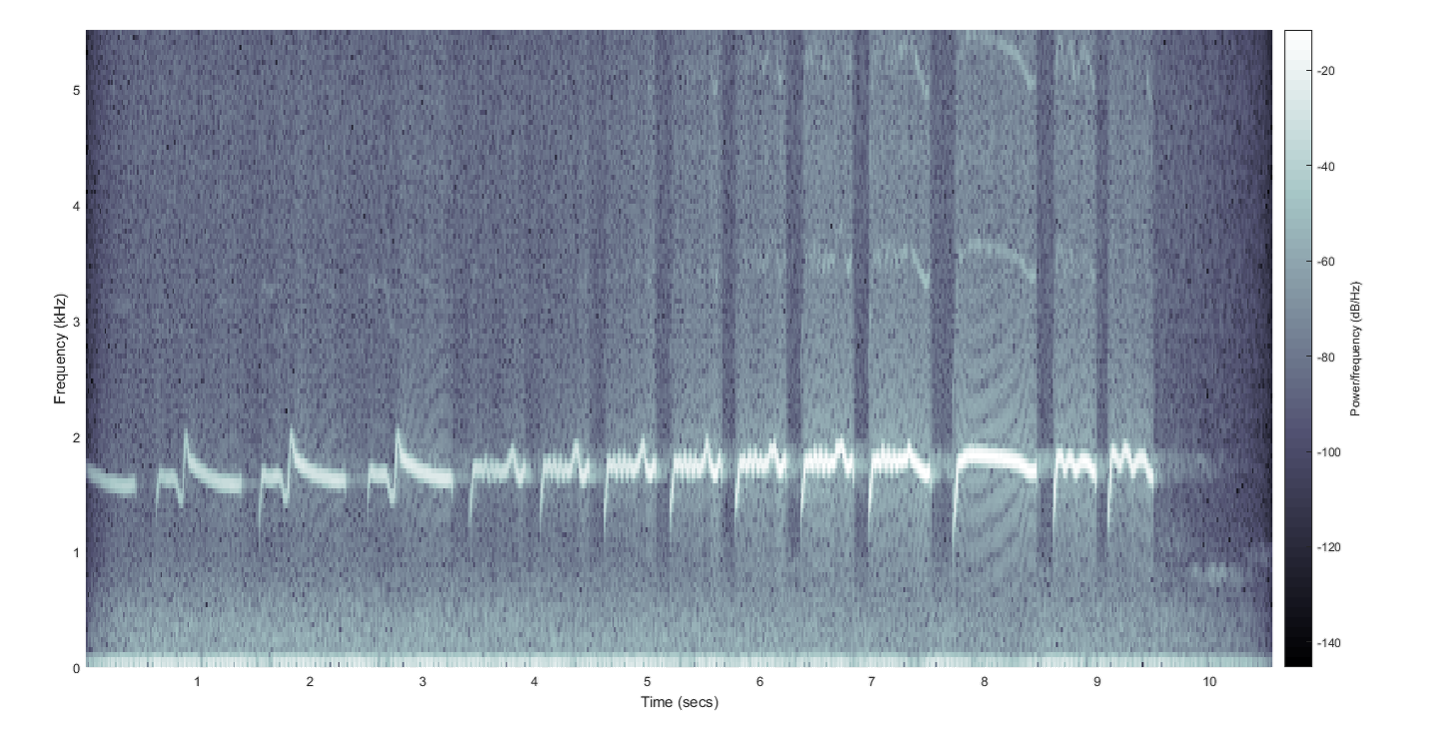
\includegraphics[width=\textwidth]{spec}
\caption{Spectrogram from a birdsong recording of the species \emph{Vanillus vanillus}.}
\label{fig_spec}
\end{figure}
\par The last concept we present in this subsection is the z-transform, which is an alternate way of mapping a discrete-time signal into its frequency-domain representation. 
\begin{definition}{Z-transform.} \label{def_ztransform}
Given a discrete-time signal $\V{x}$, its z-transform, denoted by $\mathcal{Z}\{\V{x}\}$, is given by:
\begin{align*}
X(z) = \mathcal{Z}\{\V{x}\} = \sum_{n=0}^\infty{x_nz^{-n}}
\end{align*}
\end{definition}
\par A property that will prove useful later on is called the time shifting property:
\begin{definition}{Time-shifting.} \label{def_timeshitfing}
Given a signal $\V{x}$, with z-transform $X(z)$, and a time shift-version $\V{x}'$, where $x_n = x'_{n-k}$, the z-transform of $\V{x}'$ is given by:
\begin{align*}
X'(z) = \mathcal{Z}\{\V{x}'\} = z^{-k}X(z)
\end{align*}
\end{definition}
\par Similar to the Fourer transform, the z-transform also satisfies the convolution property. In particular, given an LTI system $y_n = \sum_{-\infty}^\infty{x_kh_{n-k}}$, applying the z-transform on both sides yields $Y(z) = H(z)X(z)$, where $H(z($ is called the \emph{system function}.
\subsection{Autoregressive models and the autocorrelation function} \label{subsection_autoregression}
In this section, we describe useful statistical tools to analyse signals over time. This presentation follows closely the concepts shown in \cite{Roberts2014}, and the reader is referred to it for further details. An \emph{autoregressive model} is one that assumes that an element $x_t$ of a time series is a linear combination of previous samples, added to a random component that is assumed to be Gaussian. Autoregressive models are defined in \cite{Johnston} as follows:
\begin{definition}{p-th order Autoregressive Model.} \label{def_ar}
The \emph{p-th} order autoregressive time series (often written AR($p$)) $X_k$ is given by the following equations:
\begin{align*}
\sum_{i=0}^p{\rho_iX_{k-i}} = \epsilon_k
\end{align*}
with $\rho_0 \neq 0, \rho_p \neq 0$ and each $\epsilon_k$ is assumed to be uncorrelated and sampled from $\mathcal{N}(0, \sigma^2)$.
\end{definition}
\par In other words, at time $t$, $x_t$ is a linear combination of the $p$ previous samples, plus Gaussian noise. Notice that we can write these equations in vector form. For example, for $p=3$:
\begin{align*}
\left[ \begin{array}{c} x_4 \\ x_5 \\ .. \\ x_N  \end{array} \right] &= \begin{bmatrix} x_3 & x_2 & x_1 \\ x_4 & x_3 & x_2 \\ .. & .. & .. \\ x_{N-1} & x_{N-2} & x_{N-3} \end{bmatrix} \left[ \begin{array}{c} a_1 \\ a_2 \\ a_3 \end{array} \right] + \left[ \begin{array}{c} e_4 \\ e_5 \\ .. \\ a_N \end{array}
\right]\\
\V{x} &= \V{Ma} + \V{e}
\end{align*}
\par We can approximate $\V{a}$ by solving the last equation: $\hat{\V{a}} = (\V{M}^T\V{M})^{-1}\V{M}^T\V{X}$. Then we can approximate $\V{x}$ by letting $\hat{\V{x}} = \V{Ma}$ and then having $\V{e} = \V{x} - \hat{\V{x}}$. 
\par Another useful tool to analyse $\V{x}$ is the autocovariance, which measures how much two samples $x_t, x_{t-T}$ of the same signal change together. 
\begin{definition}{Autocovariance and autocorrelation.} \label{def_autocov}
The autocovariance with lag $T$ of a signal $\V{x}$ with mean $\mu_x$ is given by:
\begin{align*}
\sigma_{xx}(T) = \frac{1}{N-1}\sum_{i=1}^N{(x_{t-T}-\mu_x)(x_t-\mu_x)}
\end{align*}
\par The \emph{autocorrelation} is normalised version of the autocovariance, and is given by:
\begin{align*}
r_{xx}(T) = \frac{\sigma_{xx}(T)}{\sigma_{xx}(0)}
\end{align*}
\end{definition}
\par We will now establish a link between the autocorrelation and the autoregressive expansion of a signal $\V{x}$. We begin by expanding a single sample $x_t$ and multiplying it times the lagged sample $x_{t-k}$.
\begin{align*}
x_tx_{t-k} = a_1x_{t-1}x_{t-k} + a_2x_{t-2}x_{t-k} + ... + a_px_{t-p}x_{t-k} + e_tx_{t-k}
\end{align*}
\par Summing over $t$ and dividing over $N-1$ yields the autocovariance:
\begin{align*}
\sigma_{xx}(k) = a_1\sigma_{xx}(k-1) + a_2\sigma_{xx}(k-2) + ... + a_p\sigma_{xx}(k-p) + \sigma_{e,x}
\end{align*}
\par Nevertheless, the noise is assumed to be independent from the signal, and thus $\sigma_{e,x} = 0$. Normalising the expression above, we obtain the autocorrelation as a function of the autoregression coefficients $\V{a}$:
\begin{align*}
r_{xx}(k) = a_1r_{xx}(k-1) + a_2r_{xx}(k-2) + ... + a_pr_{xx}(k-p)
\end{align*}
\par For an AR($p$) model, and using the symmetry of the autocorrelation function, the relatin above can be written in matrix form:
\begin{align*}
\left[ \begin{array}{c} r_{xx}(1) \\ r_{xx}(2) \\ r_{xx}(3) \\ .. \\ r_{xx}(p)  \end{array} \right] &= \begin{bmatrix} r_{xx}(0) & r_{xx}(1) & r_{xx}(2) & .. & r_{xx}(p-1) \\ r_{xx}(1) & r_{xx}(0) & r_{xx}(1) & .. & r_{xx}(p-2) \\ .. & .. & .. & ..  & .. \\ r_{xx}(p-1) & r_{xx}(p-2) & r_{xx}(p-3) & .. & r_{xx}(0) \end{bmatrix} \left[ \begin{array}{c} a_1 \\ a_2 \\ a_3 \\ .. \\ a_p \end{array} \right]
\end{align*}
\par Or, more succintly:
\begin{align*}
\V{r} &= \V{Ra}
\end{align*}
\par This implies that the AR($p$) model coefficients for a signal $\V{x}$ can be found given its autocorrelation matrix, i.e. $\hat{\V{a}} = \V{R}^{-1}\V{r}$. This is particularly useful if we remark that $\V{R}$ is a Toeplitz matrix, i.e. its diagonals all contain the same elements, since it makes this system more efficiently solvable by means of the Levinson-Durbin recursion algorithm, which is described in subsection \ref{subsection_levinson}.
\par To finish this section, we present an interesting theorem that relates the Fourier Transform and the autocorrelation \cite{Weisstein2015c}. First, we introduce the autocorrelation $f\star f$ of a continuous function $f$ is defined as:
\begin{align*}
f \star f = \int_{-\infty}^\infty{\bar{f}(t)f(\tau + t)d\tau}
\end{align*}
\par where $\bar{f}$ denotes the complex conjugate of $f$. 

\begin{theorem}{Wiener-Khinchin Theorem.} \label{thm_wiener}
Let $\mathcal{F}\{f(t)\}(\omega) = F(\omega)$, with complex conjugate $\bar{F}$. Then, the following holds:
\begin{align*}
\mathcal{F}^{-1}\{\abs{F(\omega)}^2\}(t) &= \int_{-\infty}^\infty{\bar{f}(t)f(\tau + t)d\tau}\\
&= f \star f
\end{align*}
\end{theorem}

\par This result implies that the autocorrelation can be computed more efficiently by taking two FFT (i.e. $\mathcal{O}(n\log{n})$), rather than using the brute force approach (which is $\mathcal{O}(n^2)$).

\subsection{The Levinson-Durbin recursion} \label{subsection_levinson}
In this subsection, we present an algorithm that efficiently solves linear systems of equations when the matrix of coefficients is a Toeplitz matrix. This follows closely the work of \cite{Oppenheim2010} and \cite{Collomb2009}, thus the reader is referred to these for further details.
\par In the last subsection, we rewrote the AR($p$) coefficients as the solution to the equation $\V{r} = \V{Ra}$, where $\V{R}$ is the autocorrelation matrix. Notice that we can also write this as an homogeneous system $\V{r-Ra} = 0$. 
\par Moreover, we can expand this system by noticing that there is an additional equation satisfied by this solution, given by:
\begin{align*}
r_{xx}(0) - \sum_{k=1}^p{a_kr_{xx}(k)} = \xi^{(p)}
\end{align*}
\par where $\xi^p$ is the minimum mean-squared prediction error. This can be annexed to the previous system of equations to yield:
\begin{align*}
\begin{bmatrix} r_{xx}(0) & r_{xx}(1) & r_{xx}(2) & r_{xx}(3) & .. & r_{xx}(p) \\ r_{xx}(1) & r_{xx}(0) & r_{xx}(1) & r_{xx}(2) & .. & r_{xx}(p-1) \\ r_{xx}(2) & r_{xx}(1) & r_{xx}(0) & r_{xx}(1) & .. & r_{xx}(p-2) \\ .. & .. & .. & .. & ..  & .. \\ r_{xx}(p) & r_{xx}(p-1) & r_{xx}(p-2) & r_{xx}(p-3) & .. & r_{xx}(0) \end{bmatrix} \left[ \begin{array}{c} 1\\ -a_1 \\ -a_2 \\ -a_3 \\ .. \\ -a_p \end{array} \right] &= \left[ \begin{array}{c} \xi^{(p)} \\ 0 \\ 0 \\ 0 \\ .. \\ 0  \end{array} \right]
\end{align*}
\par In matrix form:
\begin{align*}
\V{R}^{(p)}\V{a}^{(p)} &= \V{e}^{(p)}
\end{align*}
\par Notice that the system for $p=1$:
\begin{align*}
\begin{bmatrix} r_{xx}(0) & r_{xx}(1) \\ r_{xx}(1) & r_{xx}(0) & \end{bmatrix} \left[ \begin{array}{c} 1\\ -a_1  \end{array} \right] &= \left[ \begin{array}{c} \xi^{(1)} \\ 0 \end{array} \right] \\
\end{align*}
\par can be very easily solved:
\begin{align*}
a_1 &= \frac{r_{xx}(1)}{r_{xx}(0)}\\
\xi^{(1)} &= r_{xx}(0) - a_1r_{xx}(1)
\end{align*}
\par The strategy of the Levinson-Dublin recursion is to make the solution to higher-order models a function of lower-order ones, thus recursively reducing the problem to the solution above. In other words, we assume that we have solved the problem for $p=k$, and thus we have found a vector $\V{a}^{(k)}$ that satisfies $\V{R}^{(k)}\V{a}^{(k)} = \V{e}^{(k)}$. 
\par Then, create the vector $\V{v}^{(k)}$ by appending a $0$ to  $\V{a}^{(k)}$. Simultaneously, create the vector $\V{u}^{(k)}$ by appending a quantity $\gamma^{(k)} = r_{xx}(k+1) - \sum_{j=0}^{k}a_j^{(k)}r_{xx}(k-j-1)$. That is, $\V{u}^{(k)}$ is the result of applying $\V{R}^{(k+1)}$ to $\V{v}^{(k)}$. 
\par We have now come to the key point in the derivation of the algorithm. We first notice that the system presented above can be reflected vertically; however, since $\V{R}^{(k+1)}$ is a Toeplitz matrix, flipping it vertically does not change it. This system of equations can be combined with the one presented above to get:
\begin{align*}
\V{R}^{(k+1)}\left[ \left[ \begin{array}{c} 1\\ -a_1^{(k)} \\ -a_2^{(k)} \\ .. \\ -a_p^{(k)} \\ 0 \end{array} \right] - \lambda_k\left[ \begin{array}{c} 0 \\ -a_p^{(k)} \\ -a_{p-1}^{(k)} \\ .. \\ -a_1^{(k)} \\ 1 \\ \end{array} \right] \right] = \left[ \left[ \begin{array}{c} \xi^{(k)} \\ 0 \\ 0 \\ .. \\ 0 \\ \gamma^{(k)} \end{array} \right] - \lambda_k\left[ \begin{array}{c} \gamma^{(k)} \\ 0 \\ 0 \\ .. \\ 0 \\ \xi^{(k)} \\ \end{array} \right] \right]
\end{align*}
\par According to the original system of equations, the right-hand side vector must contain zeros everywhere except for the first element. Therefore, we can make:
\begin{align*}
\gamma^{(k)} - \lambda_k\xi^{(k)} &= 0\\
\implies \lambda_k &= \frac{\gamma^{(k)}}{\xi^{(k)}}
\end{align*}
\par Therefore, for the first element of the right-hand side vector becomes:
\begin{align*}
\xi^{(k+1)} = \xi^{(k)} - \lambda_i\gamma^{(k)} = \xi^{(k)}(1-\lambda_k^2)
\end{align*}
\par For this choice, we have a vector with shape $\V{e}^{(k+1)}$. Therefore, we can state that the prediction coefficients of order $k+1$ are given by $a_j^{(k+1)} = a_j^{(k)}-\lambda_ka_{k-j-1}^{(k)}, j = 1,2,...,k$ and  $a_k^{(k)} = \lambda_k$. 
\par The original Levinson recursion solves the system of equations in $\Theta(n^2)$ operations, however more recent versions are able to solve it in $\Theta(n\log{n})$.

\subsection{Signal preprocessing} \label{subsection_preproc}
In this subsection, we describe procedures that are frequently used to preprocess signals to be analysed. In particular, we present the concepts of framing, windowing, pre-emphasis and feature scaling, all of which are useful (and often necessary) to apply the techniques discussed previously. The goal of preprocessing is to enhance the signal's features so as to make signal analysis easier and more accurate in later stages.
\par The first preprocessing technique we discuss is pre-emphasis. This technique aims at "compensating the high-frequency part that was suppressed during the sound production mechanism of humans" \cite{Jang1996}, and consists in applying a highpass filter to the original signal. A filter that is commonly applied in the literature corresponds to an AR(1) model: $x'_n = x_n - \alpha x_{n-1}, 0.95< \alpha < 0.99 $ \cite{Shimodaira2013}. This results in a signal that "sounds sharper and at a lower volume" than the original \cite{Jang1996}. 
\par Furthermore, as will be discussed in section \ref{section_lpc}, time signals are analysed in short intervals. The procedure of partitioning the signal into smaller sections is called segmentation, and the length of each segment is often given in milliseconds (ms). A discrete signal is always recorded along its sampling frequency $f_s$, which is the number of times per second a signal from the real world was sampled. Recurrent sampling frequencies include 22.5, 44.1 and 48 kHz. A concept associated to this is the Nyquist frequency $f_{\text{Nyquist}}$, which is the "highest frequency that can be coded at a given sampling rate in order to fully reconstruct the signal" \cite{Weisstein2015b}, and is given by half of the sampling frequency.
\par Once the length $l$ in seconds of each segment has been specified, we can calculate how many samples they contain by:
\begin{align*}
n_{\text{samples}} = l \* f_s
\end{align*}
\par However, performing this procedure creates discontinuities at the edges of each segment that were not originally present in the signal. As a result, the Fourier spectrum has more energy in high-frequency components \cite{NationalInstruments2015} that were not present before segmentation. This phenomenon is called spectral leakage, and its effects can be reduced by convolving the segment with a windowing function. 
\par There is a broad range of windowing functions, but two of the most well-known and frequently used are the Hamming window and the Hann window. Both are sinusoidal curves with wide peaks and low side lobes. This implies that the discontinuities at the edges of each segment are reduced, therefore reducing spectral leakage. However, the Hamming window does not quite reach zero at the lobes, and thus it does a better job of cancelling the nearest side lobe \cite{NationalInstruments2015}, at the expense of not removing all discontinuities, like the Hann window does.
\par Both windows of length $N$ are given by:
\begin{align*}
w(n) = \alpha - \beta \cos{(\frac{2\pi n}{N-1})}
\end{align*}
\par The Hamming window has values $\alpha = 0.54, \beta = 1 - \alpha = 0.46$, whereas the Hann window sets both values $\alpha = \beta = 0.5$. A comparison of both windows is shown in figure \ref{fig_windows}.
\begin{figure}[t]
\centering
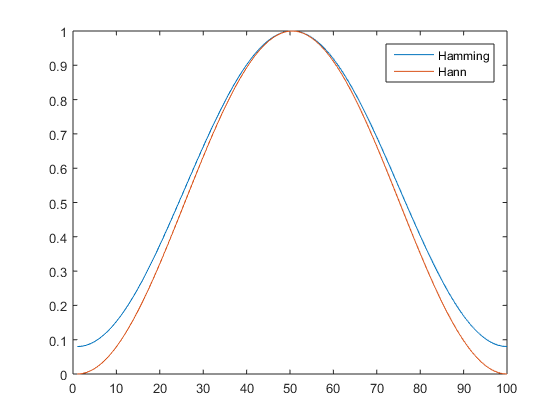
\includegraphics[width=50mm]{windows}
\caption{The Hamming window (blue) and the Hann window (orange).}
\label{fig_windows}
\end{figure}
\par The last pre-processing technique we discuss is feature scaling, or data standardisation. It consists in having our data have zero-mean and unit-variance \cite{Raschka2014}. By doing so, we guarantee that no feature will govern the computation of particular functions, and at the same time makes it easier to calculate measures such as the autocorrelation. To scale the features of the vector $\V{x}$ with mean $\mu_x$ and standard deviation $\sigma_x$, we compute:
\begin{align*}
x'_i = \frac{x_i - \mu_x}{\sigma_x}
\end{align*}
\par and use this as data instead.
\par In conclusion. pre-processing techniques enable us to perform signal analysis techniques, while at the same time enhancing the accuracy of the results. The impact of these techniques will become clearer once we have decribed the Linear Prediction of Speecg framework in the next section.

\section{Linear Predictive Coding} \label{section_lpc}
In this section, we use the tools shown in section \ref{section_dsp} to give a full description of formants. In order to do so, we present the framework of Linear Prediction of Speech, which serves as a theoretical basis to build a bridge between signal analysis and phonetics, and then introduce the concepts of formants and bandwidths. As described previously, human speech vowels and birdsong are very similar in structure, and thus using a model of speech to model birdsong is reasonable given the right assumptions. This is discussed in section \ref{subsection_lpc}.

\subsection{Linear Prediction of Speech} \label{subsection_lpc}
\par Birdsong production is done in a very similar way to human speech production. The \emph{glottis} is responsible for transmitting a signal with a flat spectrum that goes through the \emph{syrinx} (as opposed to the human larynx) \cite{Wissman2006}, which is the main part of the vocal tract of birds. The vocal tract reshapes the signal emitted by the glottis into what we hear as proper birdsong. 
\par The shape of the vocal tract changes over time, and thus birdsong, just like human speech, cannot be seen as an LTI system on the long run due to its highly changing and dynamic nature \cite{Teplitsky2000}. Nevertheless, birdsong can be seen as the output of an LTI system whose frequency response is given by the shape of the syrinx so long as the latter remains in the same state. Therefore, given a sufficiently short birdsong recording (20-50 ms), the concepts presented in section \ref{section_dsp} can be used to analyse it.
\par Now, assume that this short section of birdsong recording $\V{s}$ can be approximated by a $p$-th order autoregressive model $\hat{\V{s}} = \sum_{i=1}^pa_is_{n-i}$, as described in subsection \ref{subsection_autoregression}. Since this is only a prediction, there will be an error $\V{e}$ given by:
\begin{align*}
e_n = s_n - \hat{s}_n = s_n - \sum_{i=1}^pa_is_{n-i}
\end{align*}
\par Then, the error $\V{e}$ can also be seen as the output of an LTI system whose filter subtracts the best approximation $\hat{\V{s}}$ from $\V{s}$ \cite{Bello}. The system function can be found by taking the z-transform (and taking advantage of the time-shifting property) of the equation above:
\begin{align*}
\mathcal{Z}\{\V{e}\} &= \mathcal{Z}\{\V{s} - \hat{\V{s}}\}\\
E(z) &= \mathcal{Z}\{\V{s}\} - \mathcal{Z}\{ (\sum_{i=1}^pa_ix_{n-i})_n\} \\
 &= S(z) - S(z)\sum_{i=1}^pa_iz^{-i}\\
 &= S(z)(1 - P(z))\\
 &= S(z)A(z) 
\end{align*}
\par where $A(z) = 1 - \sum_{i=1}^pa_iz^{-i}$. Now, consider the LTI system with input $\V{e}$, output $\V{s}$ and system function $H(z)$. If this output were to be used as input to the system described above, then we should recover $\V{e}$. This implies that both system functions are mutually inverse, i.e. $H(z)A(z) = 1$, and therefore $H(z) = 1/A(z)$. 
\par Now assume that $\V{e}$ is the signal emitted by the glottis. Then, the LTI system described in the above paragraph can be used to model birdsong production, which implies that the vocal tract can be characterised by the system function:
\begin{align*}
H(z) = \frac{1}{A(z)} = \frac{1}{1-\sum_{i=1}^pa_iz^{-i}}
\end{align*}
\par We bring the reader's attention to the fact that $H(z)$ is fully characterised by the parameters $\{a_i\}$, which can be found by performing a linear prediction analysis as described in section \ref{section_dsp}. Therefore, we have now built a bridge between signal analysis and phonetics, which can be summarised as: the linear prediction coding (LPC) coefficients  $\{a_i\}$ model the filter the syrinx applies to the signals emitted by the glottis. We recall that finding the LPC coefficients can be done purely by analysing the output signal $\V{s}$, and thus we have all that is required to perform it.
\subsection{Formants} \label{subsection_fmnts}
\par In this section, we use the framework of linear prediction of speech to define formants. In subsection \ref{subsection_lpc}, we described the LTI system analogous to birdsong production, and showed that the system function $H(z)$ is given by:
\begin{align*}
H(z) = \frac{1}{1 - \sum_{i=1}^pa_iz^{-i}} = \frac{1}{A(z)}
\end{align*}
\par We are now ready to present formants:
\begin{definition}{Formants.} \label{def_formants}
In the Linear Prediction of Speech framework, the formants of a signal are the resonances of the vocal tract, i.e. the frequencies associated with the poles of the system function $H(z)$ \cite{Snell1993}. In other words, given a pair of complex roots $re^{\abs{\theta}}$, the formant frequency associated to it is given by:
\begin{align*}
F = \frac{f_s}{2\pi}\theta \text{Hz}
\end{align*}
\end{definition}
\par where $f_s$ is the sampling frequency of the signal. 
\par Formants can be visualised as the peaks of the frequency response of the LTI system, as depicted in figure \ref{fig_fmnts_lpc}. In this plot, we can also observe the 3-dB bandwidth of each formant. 
\begin{definition}{3-dB bandwidth.}\label{def_bandwidth}
The 3-dB bandwidth of a formant is defined as the length of the interval the spectral envelope occupies 3-dB below the peak associated to the chosen formant. Given a pair of complex roots $re^{\abs{\theta}}$, the bandwidth associated to it is:
\begin{align*}
B = -\frac{f_s}{2\pi}\log{r} \text{Hz}
\end{align*}
\end{definition}
\begin{figure}[t]
\centering
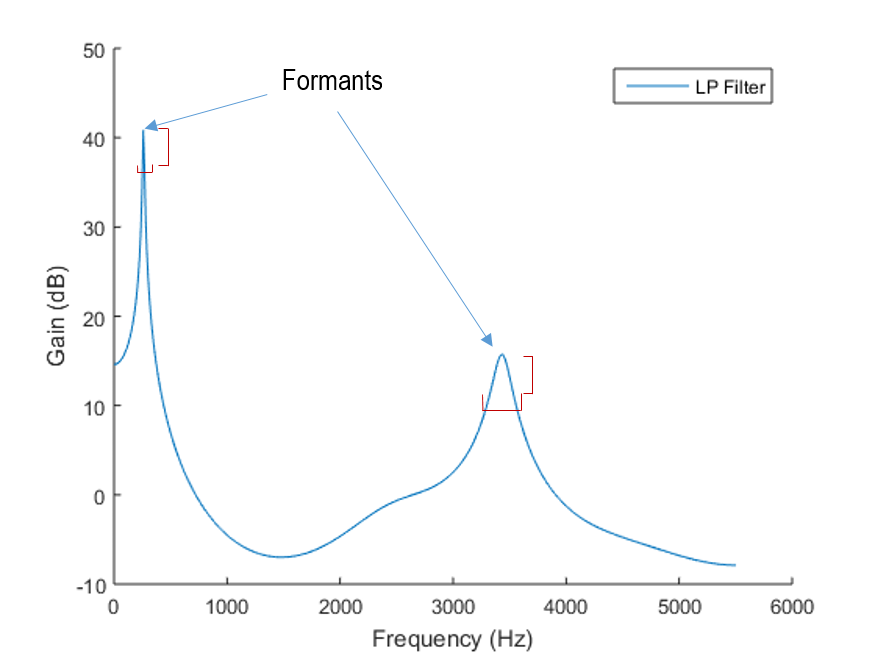
\includegraphics[width=\textwidth]{formants_envelope}
\caption{Given an LTI system, its formants are the peaks of its spectral envelope. The bandwidth associated to each formant are depicted as red boxes next to each peak.}
\label{fig_fmnts_lpc}
\end{figure}
\par This definition suggests that a narrower bandwidth implies a "peakier" formant, i.e. a particular frequency that contains more energy in a shorter interval. This implies that more characteristic formants are those with narrower bandwidths.
\par To wrap up, recall that this analysis is being done for a single instant of time, i.e. for a window of 20-50 ms of birdsong. Done in the long run, we can estimate a full trajectory of formants for each recording, and use it as a vector of features. This trajectory can be visualised in spectrograms, as depicted in figure \ref{fig_specformants}.
\begin{figure}[t]
\centering
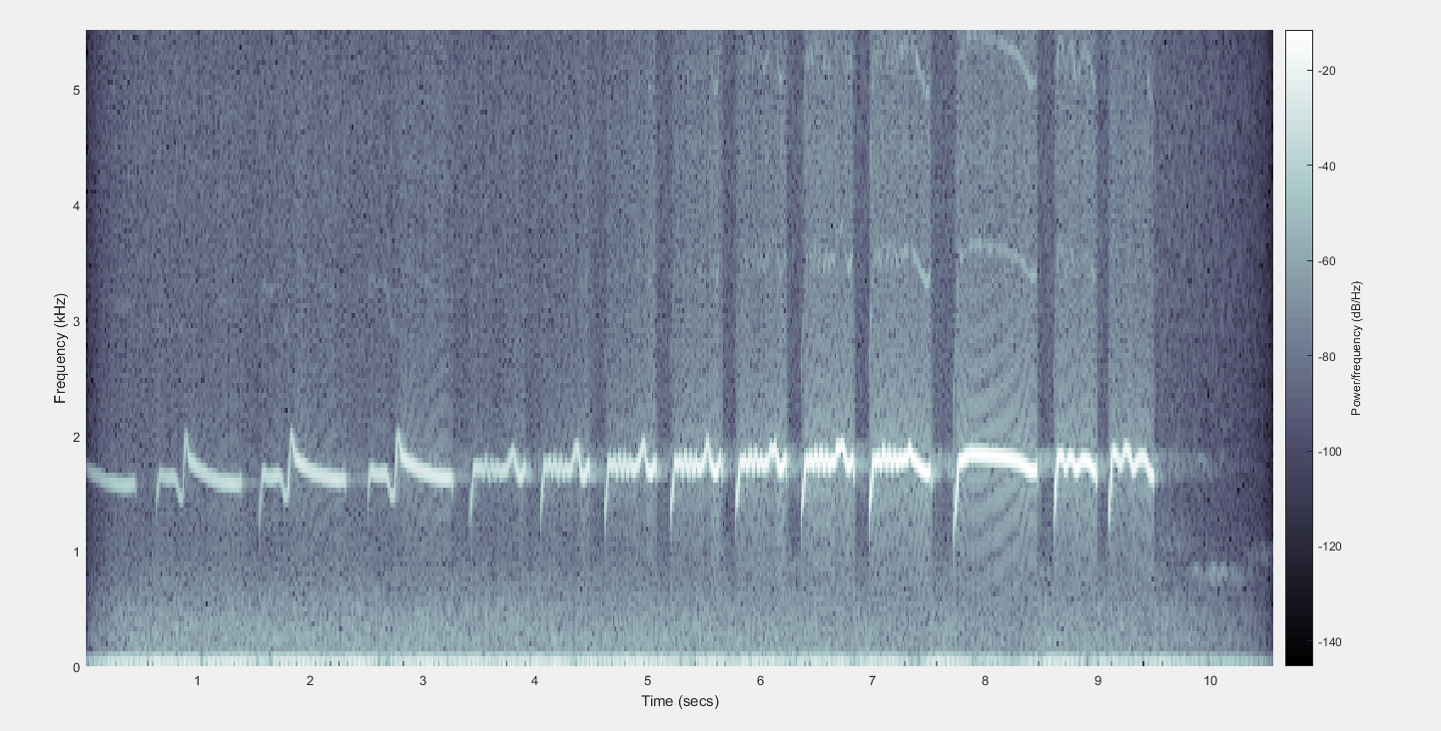
\includegraphics[width=\textwidth]{formants}
\caption{Formant trajectories are the white bars that can be spotted on spectrograms. }
\label{fig_specformants}
\end{figure}


\section{Conclusion} \label{section_form_estimation}
To wrap up, in this section we presented the Linear Prediction of Speech framework, its relationship with birdsong production and the required DSP techniques. As discussed, formants can prove to be useful features due to its close relationship with human speech vowels. However, some issues still remain, particularly: is formant trajectory extraction sufficient to fully characterise each bird species? How are trajectories of different length to be handled? How about stretched or shifted versions of the same kind of birdsong? 
\par These factors justify going one step ahead from here and try to characterise the formant trajectories of bird species into objects that are comparable and invariant to the transformations mentioned above. In consequence, methods to further characterise the extracted formant trajectories will be presented in chapter \ref{chapter_hmms}. 
    

\end{document}